\documentclass{statphysicsdep}



%%%%%%%%%%%%%%%%%%%%%%%%%%%%%%%%%%%%%%%%%%%%%%%%%%%%%%%%%%%%%
% Настройки титулки
\usepackage{unn-titlepage}
\TitleWorkTitle{Метод компенсации нелинейных искажений усилителя мощности для стандарта мобильной связи 5G NR}

\setauthor{1}{Зав. кафедрой статистической радиофизики  \\ и мобильных систем связи,  \\ профессор, д.ф.–м.н.}{Мальцев А.А.}
\setauthor{2}{Научный руководитель,  \\ профессор, д.ф.-м.н}{Мальцев А.А.}
\setauthor{3}{Рецензент,  \\ профессор, д.ф-м.н.}{Морозов О.А.}
\setauthor{4}{Консультант по технике безопасности,  \\ доцент, к.ф.-м.н.}{Клемина А.В.}
\setauthor{5}{Студент 4-го курса магистратуры}{Шиков А.П.}
%%%%%%%%%%%%%%%%%%%%%%%%%%%%%%%%%%%%%%%%%%%%%%%%%%%%%%%%%%%%%


% Для псевдокода
%%%%%%%%%%%%%%%%%%%%%%%%%%%%%%%%%%%%%%%%%%%%%%%%%%%%%%%%%%%%%
\usepackage{algorithm}
\usepackage{algpseudocode} 
\floatname{algorithm}{Алгоритм}
%%%%%%%%%%%%%%%%%%%%%%%%%%%%%%%%%%%%%%%%%%%%%%%%%%%%%%%%%%%%%

% Настройки номенклатуры
%%%%%%%%%%%%%%%%%%%%%%%%%%%%%%%%%%%%%%%%%%%%%%%%%%%%%%%%%%%%%
\usepackage{nomencl}
\usepackage{multicol}
\usepackage{etoolbox}
\renewcommand\nomgroup[1]{%
\item[\bfseries
\ifstrequal{#1}{A}{Сокращения}{%
\ifstrequal{#1}{B}{Обозначения}{%
\ifstrequal{#1}{C}{}{}}}%
]}
\newcommand{\nomunit}[1]{%
\renewcommand{\nomentryend}{\hspace*{\fill}#1}}
\renewcommand{\nompreamble}{\footnotesize\begin{multicols}{2}}
\renewcommand{\nompostamble}{\end{multicols}}
\renewcommand{\nomname}{Обозначения и сокращения}
\makenomenclature  
\makeindex
%%%%%%%%%%%%%%%%%%%%%%%%%%%%%%%%%%%%%%%%%%%%%%%%%%%%%%%%%%%%%

% \usepackage{booktabs} % For \toprule, \midrule and \bottomrule
% \usepackage{siunitx} % Formats the units and values
% \usepackage{pgfplotstable} % Generates table from .csv
% \pgfplotsset{compat=1.18}
% \usepackage{tabularx}
% % Setup siunitx:
% \sisetup{
%   round-mode          = places, % Rounds numbers
%   round-precision     = 2, % to 2 places
% }






% Прочее
\newcommand\mean[1]{\langle #1 \rangle}
\newcommand\const{\text{const}}
\renewcommand{\phi}{\varphi}
\renewcommand{\epsilon}{\varepsilon}
\renewcommand\vec[1]{\vectorbold{#1}}
\setcounter{MaxMatrixCols}{20}

% Настройка переносов некоторых слов
\hyphenation{при-ем-ни-ков}

\addbibresource{library.bib}
\usepackage{enumitem}
\usepackage{subcaption}
\usepackage{soulutf8}

\makeatletter
\patchcmd{\@setref}{\bfseries ??}{\bfseries\hl{??}}{}{}
\makeatother

% \titlecontents{chapter}[0pt\addvspace{15pt}]
% {\llap{\makebox[3em]{\oldstylenums{\thecontentspage\hfill\thecontentslabel}}\hskip1em}
%   \small\scshape\vskip-\baseline{}skip}{}{}{}
% \titlecontents*{section}[20pt]
% {\upshape}{}{}
% {, \oldstylenums{\thecontentspage}}[][\ \textbullet\ ][]

\def\ACS{\textit{ACS}}
\def\baseline{\textit{baseline}}
\def\hSearchMMSE{\textit{hSearchMMSE}}
\def\AuxBeam{\textit{AuxBeam}}

% \newcommand{\ACS{}}{{ACS}~}
% \newcommand{\baseline{}}{{baseline}~}
% \newcommand{\hSearchMMSE{}}{{hSearchMMSE}~}
% \newcommand{\AuxBeam}{{AuxBeam}~}

\makeatletter
\patchcmd{\@setref}{\bfseries ??}{\bfseries\hl{??}}{}{}
\makeatother
\begin{document}



\maketitle
\newpage

\small
{
\hypersetup{linkcolor=black}
\tableofcontents
}
\normalsize

\nomenclature[A]{LLS}{Link Level Simulator}
\nomenclature[A]{УМ}{Усилитель Мощности}
\nomenclature[A]{КУ}{Коэффициент Усиления}
\nomenclature[A]{АХ}{Амплитудная Характеристка}
\nomenclature[A]{ФХ}{Фазовая Характеристка}
\nomenclature[A]{OBO}{Output Back-Off}
\nomenclature[A]{IBO}{Input Back-Off}
\nomenclature[A]{5G NR}{5G New Radio}
\nomenclature[A]{OFDM}{Orthogonal Frequency Division Multiplexing}
\nomenclature[A]{CP}{Cyclic Prefix}
\nomenclature[A]{PD}{Pre-Distortion}
% \nomenclature[A]{AATLF}{Adaptive Angle Tracking Loop Filter}
% \nomenclature[A]{AIC}{Akaike’s Information Criterion}
% \nomenclature[A]{AIP}{Antenna in Package}
% \nomenclature[A]{AOA}{Angle of Arrival}
% \nomenclature[A]{AOD}{Angle of  Departure}
% \nomenclature[A]{AWGN}{Additive White Gaussian Noise}
% \nomenclature[A]{BRP}{Beam Refinement Protocol}
% \nomenclature[A]{CCATLF}{Constant Coefficient Angle Tracking Loop Filter}
% \nomenclature[A]{CDF}{Cumulative Distribution Function}
% \nomenclature[A]{CFAR}{Constant False Alarm Ratio}
% \nomenclature[A]{CoMP}{Coordinated Multipoint}
% \nomenclature[A]{CSI}{Channel State Information}
% \nomenclature[A]{DCO}{Digitally Controlled Oscillator}
% \nomenclature[A]{DKED}{Double Knife-Edge Diffraction}
% \nomenclature[A]{DVR}{Digital Video Recorder}
% \nomenclature[A]{EG}{Equal Gain}
% \nomenclature[A]{EKF}{Extended Kalman Filter}
% \nomenclature[A]{FFT}{Fast Fourier Transform}
% \nomenclature[A]{GCS}{Global Coordinate System}
% \nomenclature[A]{HBF}{Hybrid Beamforming}
% \nomenclature[A]{HDTV}{High Definition Television}
% \nomenclature[A]{KF}{Kalman Filter}
% \nomenclature[A]{LCS}{Local Coordinate System}
% \nomenclature[A]{LF}{Loop Filter}
% \nomenclature[A]{LOS}{Line-of-Sight}
% \nomenclature[A]{MDL}{Minimum Description Length}
% \nomenclature[A]{ML}{Maximum Likelihood}
% \nomenclature[A]{MMSE}{Minimal Mean Square Error}
% \nomenclature[A]{MPM}{Minimal Polynomial Method}
% \nomenclature[A]{MS}{Maximal Selection}
% \nomenclature[A]{MUSIC}{MUltiple SIgnal Classification}
% \nomenclature[A]{MVDR}{Minimum Variance Distortionless Response}
% \nomenclature[A]{NLOS}{Non Line-of-Sight}
% \nomenclature[A]{NR}{New Radio}
% \nomenclature[A]{PBCH}{Physical Broadcast Channel}
% \nomenclature[A]{PDF}{Probability Density Function}
% \nomenclature[A]{PSS}{Primary Synchronization Signal}
% \nomenclature[A]{RGB-D}{Red-Green-Blue-Depth}
% \nomenclature[A]{RS}{Reference Signal}
% \nomenclature[A]{SLS}{Sector Level Sweep}
% \nomenclature[A]{SSS}{Secondary Synchronization Signal}
% \nomenclature[A]{SVD}{Singular Value Decomposition}
% \nomenclature[A]{TDM}{Time Division Multiplexing}
% \nomenclature[A]{ULA}{Uniform Linear Array}

\printnomenclature
\newpage

%! TeX root = ../main.tex
\Introduction

Развитие стандарта мобильной связи 5G New Radio (NR), разрабатываемого консорциумом
3GPP (3rd Generation Partnership Project), тесно связано с развитием
технологии Интернета Вещей (IoT - Internet of Things). Высокая скорость,
надежность сети, малая задержка, а также возможность массового подключения
"умных" устройств являются важнейшими параметрами, определяющими
производительность системы в целом.

Одни из последних релизов стандарта 5G NR - релизы 15 и 16 обеспечивают
поддержку несущих частот до 52.6 ГГц. С целью расширить поддержку текущего
частотного диапазона FR2 (\textit{Англ. - Frequency Range 2}) до 52.6 - 71 ГГц с
минимальными вносимыми изменениями в систему \cite{intel193259}
\cite{qlcm193229}, группа RAN проекта 3GPP уже исследовала требования для
диапазона 52.6 - 114.25 ГГц \cite{3gpp.38.807}. Помимо этого, была также
исследована возможность расширения частотного диапазона до миллиметровых
волн 71-114 ГГц. Однако в этом диапазоне появляется такое ограничение, как
нелинейный искажения, вызванные работой усилителя мощности (УМ). Несмотря
на значительное продвижение в технологии разработки и проектирования УМ с
использованием новых материалов, все ещё наблюдаются значительные нелинейные
искажения сигнала при использовании стандартной мощности передатчика
\cite{zhang2021}. В данном диапазоне частот УМ может внести значительные
искажения, кардинально снизив производительность
системы. Это особенно заметно для высокоэффективных модуляций, например,
64-QAM и 256-QAM.

Данным эффектом искажения сигнала можно пренебречь в низких диапазонах
частот, таких как FR1 и частично FR2. Рабочую точку УМ в этих диапазонах
можно выбрать таким образом, что на выходе усилителя будет достигаться
необходимая выходная мощность, и при этом УМ будет работать в линейной
области своей характеристики, что минимизирует вносимые в передаваемый
сигнал искажения.

Проблема искажения сигнала на высоких частотах наиболее актуальна а рамках
рассмотрения использования стандарта связи 5G NR в применении к технологии
Интернета Вещей. В данном случае система имеет огромное количество
небольших и простых передающих устройств, таких как датчики, сенсоры, а
также прочие устройства, используемые для обеспечения тесно
связанного окружения. Подобные элементы часто имеют низкокачественные
передающие и усилительные цепи ввиду необходимости общей низкой стоимости
прибора. Также данные устройства должны быть энергоэффективными и
минимизировать общее потребление электроэнергии для возможности создания
инфраструктуры из большого количества отдельных компонент.
Эти факторы являются ключевыми при выборе метода компенсации вносимых
нелинейных искажений, поскольку вспомогательная обработка на передатчике
может внести дополнительные энергозатраты, нежелательные для дешевого,
энергоэффективного устройства.

Проблема компенсации нелинейных искажений, вносимых УМ, рассматривалась во
многих работах, в том числе для низких диапазонов частот
\cite[]{sharath2015,shabany2008,eda2001,maltsev2021,bhat2016,qi2010,gregorio2007}.
Рассматривались различные подходы, в основе которых лежали предварительное
искажение (\textit{Англ. - Pre-Distortion (PD), Digital Pre-Distortion
(DPD)}) сигнала на передатчике с целью "выпрямления" амплитудной
характеристики усилителя. Однако такие методы требуют дополнительной
сигнальной обработки на передатчике, что негативно влияет на
энергоэффективность устройства. В основе другого метода лежит обработка
сигнала на приемнике, когда принятый сигнал подвергается обработке на
стороне принимающего устройства с целью компенсации искажений, внесенных на
УМ передатчика. В качестве методов компенсации используют обратную
характеристику УМ, статистические подходы для определения усредненного
искажения и его дальнейшей компенсации, последовательный метод Монте-Карло
и другие. Также важно отметить необходимость в определенных случаях знать
на приемнике параметры УМ, который расположен на передатчике.

Также важно отметить, что характеристики УМ в миллиметровом диапазоне
частот 100-200 ГГц значительно отличаются от характеристик усилителей в
диапазоне 30-70 ГГц. На более высоких частотах, характеристики значительно
хуже, это означает необходимость применения определенного метода
компенсации искажения для повышения качества передачи информации.

В данной работе предлагается метод компенсации нелинейных искажений
внесенных усилителем мощности на приемнике. Основа метода компенсации
заключается в использовании обратной характеристики УМ, однако перед этим
сигнал определенным образом обрабатывается. Предлагаемый метод может быть
использован для разных типов сигналов(CP-OFDM, DFT-s-OFDM),
в зависимости от рассматриваемой задачи. Также, в рамках данной работы были
исследованы характеристики современных твердотельных УМ в миллиметровом диапазоне. На
основе проведенного исследования, была создана модель для диапазона
частот 100-200 ГГц, которая в дальнейшем использовалась в математическом
моделировании для проверки работоспособности предлагаемого метода.



% \textbf{Черновой план диплома}

% \textit{Краткое описание. Скорее для себя, чтобы самому не забыть в чем
% основная суть работы, в дипломе этого не будет}

% \begin{itemize} \item 5G расширяется и активно исследует суб-ТГц диапазон
%     \item усилители в этом диапазоне не очень, много искажений
%     \item особенно для маленьких дешевых устройств, где важна
%     энергоэффективность
%     \item нужна обработка на приемнике
%     \item предлагаемый метод обработки
%     \item краткий план-содержание работы
%     \end{itemize}





% Дипломная работа о разработке метода компенсации нелинейных искажение
% сигнала на приемнике, возникших в результате работы усилителя мощности на
% передатчике. Усилитель имеет нелинейную амплитудную характеристику, что и
% является причиной искажения сигнала.

% Учитывая планы расширения стандарта 5G в суб-терагерцовый диапазон,
% нелинейность характеристики УМ в этих частотах только ухудшается,
% значительно снижая эффективность системы в целом. Это является основным
% мотивом разработки метода компенсации вносимых передатчиком искажений на
% приемнике.

% Также, компенсация рассматривается именно на приемнике, поскольку в таком
% случае передатчику не нужно производить дополнительную обработку сигнала,
% что важно для энергопотребления. Такой метод может использоваться в
% системах с большим количеством мало-размерных, простых передатчиков,
% которые часто используются в системе интернета вещей.

% \section{Введение (5G, IoT, sub-THz range, PA nonlinearity)}


% \section{Роль усилителя мощности и влияние нелинейности амплитудной
% характеристики} \subsection{Описание принципа работы усилителя мощности}
% \subsection{Влияние нелинейности и искажение различных сигналов на
% приемнике} \subsubsection{Искажение сигнала SC} \subsubsection{Искажение
% сигнала CP-OFDM} \subsubsection{Искажение сигнала DFT-s-OFDM}
% \subsection{Характеристики усилителей в суб-ТГц диапазоне}
% \subsection{Обзор существующих моделей для описания усилителя мощности}
% \subsubsection{Модель Rapp} \subsubsection{Новая модель для диапазона
% частот 100-200 ГГц}

% \section{Метод компенсации нелинейных искажений на приемнике}
% \subsection{Краткое описание принципа работы симулятора канального
% уровня} \subsection{Подход и описание нового метода компенсации
% нелинейных искажений} \subsubsection{Адаптация алгоритма компенсации в
% зависимости от типа используемого сигнала} \subsubsection{Компенсация с
% использованием обратной характеристики усилителя}

% \section{Результаты расчетов и симуляций} \subsection{Модель усилителя
% мощности в диапазоне 30-70 ГГц} \subsection{Модель усилителя мощности в
% диапазоне 100-200 ГГц}

% \section{Заключение}

% \section{Приложение}

% \newpage
% \Introduction

% \textit{В введении указывается актуальность темы, цели и задачи исследования, предметы и
% методы исследования, теоретическую и практическую значимость, научная новизна,
% положения, выносимые на защиту, краткое описание структуры работы.}


% В последние годы Интернет Вещей (IoT), поддерживаемый технологией 5G,
% стремительно развивался в широком спектре применений, обеспечивая связь
% между объектами в автомобильной индустрии, бытовой электронике,
% транспортном, логистическом и производственном секторе. С ростом
% повсеместной интеграции и использования различных малогабаритных
% датчиков, стоимость производства каждого отдельно взятого элемента
% остается критическим аспектом. Относительно низкая цена отдельных
% элементов является ключом к созданию тесно связанной среды, однако это
% может серьезно повлиять на качество радиочастотных цепей, а также на
% общую производительность системы. С расширением 5G до субтерагерцовых
% диапазонов, нелинейные искажения усилителя мощности (УМ) могут
% значительно ограничить производительность системы даже в
% высококачественных устройствах из-за конструктивных ограничений
% усилителя. Было проведено множество исследований с целью уменьшения
% влияние нелинейности как на стороне передатчика, так и на стороне
% приемника. Многие решения предлагают определенные варианты оценки
% эффектов УМ посредством обратной связи, направленной на принятие решения,
% обучения или даже статистической обработки полученного сигнала. Однако,
% зная функцию нелинейности УМ на приемной стороне, обработка может быть
% упрощена до применения обратной функции к эквивалентному сигналу во
% временной области.

% В этой работе мы предлагаем метод компенсации нелинейных искажений УМ на
% стороне RX, который можно настроить для нескольких форм сигналов, таких
% как CP-OFDM и DFT-S-OFDM. Приведенные результаты моделирования
% демонстрируют улучшение характеристик как для субтерагерцовых моделей УМ,
% так и для моделей в диапазоне 30-70 ГГц со значительно лучшими
% характеристиками.



% \section{Описание проблемы и предшествующие решения}
% \textbf{введение из статьи}

% Последние релизы стандарта 5G New Radio (NR) Rel15 и Rel16 поддерживают
% частоты несущих до 52.6 ГГц. Рассматривая работу на частоте свыше 52.6
% ГГЦ, группа RAN проекта 3GPP уже  исследовала требования для диапазона
% частот 52.6 – 114.25 ГГЦ [1], с основной целью расширить  поддержку
% текущего диапазона NR FR2 до 52.6-71 ГГЦ с минимальными изменениями в
% системе [2][3]. Также были исследованы возможности дальнейшего расширения
% в суб-терагерцовый диапазон 71-114 ГГц. В этом диапазоне, несмотря на
% значительное продвижения в технологии разработки и создания УМ, все еще
% наблюдается сильные нелинейные искажения для стандартной разрешенной
% мощности передатчика [4]. Таким образом, искажения, вносимые усилителем
% мощности, могут значительно ограничить производительность системы,
% особенно для высокоэффективных модуляций, таких как 64- и 256-QAM.

% В низких диапазонах частот 5G NR, FR1 и частично FR2, нелинейными
% эффектами УМ можно пренебречь в большинстве случаев, поскольку рабочая
% точка может быть расположена в линейной области, позволяя минимизировать
% искажения передаваемого сигнала. Рассматриваемая проблема значительно
% более актуальна для дешевых трансиверов с низкокачественными
% усилительными цепями. Следует заметить, что количество таких устройств
% может быть очень большим, поскольку дешевые устройства обычно
% используются для создания инфраструктуры Интернета вещей. Данная проблема
% была рассмотрена в нескольких работах [5]-[11], даже для низкочастотных
% диапазонов.

% Для описания искажения амплитуды и фазы при использовании твердотельных
% усилителей мощности широко используется модель Раппа. Модифицированная
% модель Раппа, приведенная в уравнении (1), также включена в базовые
% модели спецификации 3GPP \cite{spec38807}.

% \begin{equation} a=b \end{equation}

% насыщения. A,B,q – параметры кривой искажения фазы. is the small signal
% gain, p is the smoothness factor and ?Vsat is the saturation
% voltage/A?B?qare phase distortion curve parameters.

% Базовые характеристики стандартных УМ в диапазоне частот 30-70 ГГц были
% использованы для вывода математической модели [15], справедливой в
% соответствующей полосе. Однако основываясь на недавних работах
% [4][16][17], можно отметить что характеристики Суб-ТГц УМ даже в полосе
% частот 100-200 ГГц значительно отличаются. Для оценки производительности
% системы для данного диапазона несущих частот, нами была выведена
% усредненная модель УМ на основ последних исследований. Сравнение моделей
% приведено на Figure 1. Основываясь на усредненных параметрах ???, была
% получена модель УМ для диапазона частот 100-200 ГГц.

% На Figure 2 приведены примеры искажения сигнала в следствии действия
% нелинейности УМ для разных видов сигнала. Можно отметить, что для сигнала
% с одной несущей (single carrier - SC), искажения носят детерминированный
% характер в виде амплитудного искажения, которое можно с относительной
% легкостью компенсировать. Однако для сигнала OFDM, нелинейность УМ
% приводит к интерференции между несущими, что результирует в случайном
% характере искажения, которое намного сложнее компенсировать.

% DFT spread OFDM (DFT-s-OFDM) представляет некую промежуточную ситуацию,
% когда присутствуют как и детерминированный характер искажения, так и
% случайный, позволяя произвести компенсацию нелинейности.

% На данный момент существуют два различных подхода для компенсации
% нелинейности УМ. Первый заключается в предварительном искажении сигнала
% перед УМ на передатчике, придавая сигнал определенные свойства,
% минимизирующие влияние нелинейного искажения от УМ. Существует множество
% вариантов обработки для данного подхода, однако все они имеют слабый
% эффект на общей производительности системы, а предварительное искажение
% имеет низкую эффективность на низких значениях IBO [5][6][7].
% Использование предварительного искажения  на передатчике нежелательно и
% на мало-габаритных устройствах, поскольку в этом случае растет объем
% сигнальной обработки, что увеличивает энергопотребление.

% Второй подход заключается в компенсации нелинейных искажений на
% приемнике. Например, в [8] используется статистическая обработка
% принятого сигнала для определения средней степени искажения, что
% используется для дальнейшей компенсации. Работы [5][6][9][10][11][12][13]
% рассматривают теоретический подход для компенсации на приемнике в очень
% обобщенном случае. Несколько методов компенсации влияния нелинейности УМ
% были предложены для OFDM сигнала [11][12][13], где влияние нелинейности
% представляется постоянным комплексным множителем, а также Гауссовой
% шумовой компонентой. Основной задачей в таком случае является определение
% параметров УМ (могут быть как известны изначально, так и определены с
% помощью пилотных сигналов) для компенсации нелинейного искажения.
% Несколько методов были использованы для сигнала SC с одной несущей
% [5][6][9][10], включая….??..., последовательный метод Монте-Карло, а
% также обратную характеристику УМ. В нескольких случаях [9][11][10],
% значения параметров УМ считаются известными на приемнике, что позволяет
% произвести компенсацию искажения. В случаях, когда параметры УМ
% оцениваются, производительность такая же либо хуже.

% \section{Новая идея}

% Как было показано для сигнала SC, и, не менее важно, для сигнала
% DFT-s-OFDM, искажения в результате влияния нелинейности УМ имеют
% детерминированный характер, в добавок к ICI. Зная нелинейную
% характеристику, становится возможным компенсировать детерминированную
% компоненту искажений, улучшая итоговую демодуляцию. Этого можно добиться
% применяя обработку сигнала на приемнике, эквивалентную обратной
% характеристике УМ.

% Обычно, эта функция не известна на приемнике не только потому что
% значения параметров УМ не известны, но и в следствии различных значений
% мощности передатчика. Значение этой мощности напрямую влияет на рабочую
% точку УМ, а значит и на то, как искажается конечный сигнал.

% В нескольких работах [10][11][12], the decision-directed feedback??
% используется для оценки характеристики усилителя мощности. Также, в [8]
% используется статистическая обработка для корректировки алгоритма
% демодуляции принятого искаженного сигнала.

% Однако, более эффективным подходом является использование знаний о
% параметрах УМ, а также его рабочей точки для соответствующей пост
% обработки.

% \subsection{Предлагаемый метод компенсации на приемнике} Ниже приведен
% метод компенсации нелинейных искажений УМ на стороне приемника для
% сигнала CP-OFDM, основанный на использовании обратной амплитудной
% характеристики УМ (Figure 3). 

% Схема компенсации состоит из базовой обработки на передатчике (1),
% которая может включать MIMO прекодинг и transform прекодинг (в случае
% DFT-s-OFDM сигнала),  а также стандартного для OFDM блока обратного
% преобразования Фурье. Сгенерированный OFDM сигнал подается на одну или
% более передающих цепочек, которые могут включать добавление цикличного
% префикса, перенос сигнала на несущую частоту, и, наконец, сигнал подается
% на усилитель мощности (2), работающий на несущей частоте. Отметим, что
% для корректной работы предлагаемой схемы, сигналы на разных антеннах
% должны иметь одинаковую амплитуду (но могут иметь разную фазу). Это
% ограничивает применение данного метода до передачи 1 ранга, даже если
% используется несколько передающих антенн. После прохождения через канал,
% сигнал попадает на приемную цепь состоящую из одной или нескольких
% приемных антенн для дальнейшей обработки (4), которая может состоять из
% преобразования Фурье further maximum ration combining (MRC) and frequency
% domain equalization???. Такая обработка эффективно нивелирует влияние
% частотно-селективного канала, что позволяет использовать обработанный
% сигнал на блоке компенсации нелинейного искажения (5). Этот блок может
% состоять из операции обратного Фурье преобразования (6) для возвращения
% сигнала во временную область, блока обратной нелинейной функции УМ (7),
% который выполняет компенсацию нелинейного искажения, а также блока
% прямого преобразования Фурье для возвращения сигнала в частотную область.

% \subsection{Предположения и результаты симуляции} Для проверки
% эффективности предлагаемого метода, были произведены симуляции канального
% уровня, в которых предложенный метод сравнивался со случаями идеального
% УМ, а также отсутствии компенсации на приемнике для совпадающей модели
% усилителя. Использовалась модель основанная на параметрах существующих
% усилителей мощности в диапазоне частот 30-70 ГГц [15], а также модель для
% 100-200 ГГц полученная в результате данной работы. Расчеты проводились
% для различных параметров системы, таких как расстояние между поднесущими
% (SCS), типом используемого сигнала, кодирование, модуляция и другие.
% Полный список параметров симуляции приведен в Table 1.

% \subsection{Последовательность применения компенсаций} Предложенный метод
% предполагается использовать до компенсации фазового шума (PN), однако
% другие последовательности были рассмотрены и рассчитаны. Применение
% компенсации нелинейности УМ после компенсации PN показало определенное
% ухудшение производительности, поэтому компенсация нелинейности УМ везде
% производилась до компенсации фазовых шумов в большинстве расчетов.
% Примеры результатов, в которых сравнивается разный порядок компенсации
% фазовых шумов и нелинейности усилителя приведены на Figure 10.

% \subsection{Наблюдения}

% • Для модели УМ в диапазоне 30-70 ГГц (подходящего для диапазона АК2 и
% выше) улучшение наблюдается только для модуляций высокого порядка o Для
% SCS 120 кГц, отрицательные эффекты фазового шума значительны, и при таких
% искажениях результаты компенсации нелинейности УМ незначительны o Для SCS
% 480 и 960 кГц, в которых возможна более эффективная компенсация фазового
% шума, в определенный момент влияние нелинейности УМ становится основным
% ограничивающим фактором. В этом случае компенсация нелинейности УМ может
% улучшить результат на несколько дБ или совсем избавиться от искажений,
% внесенных УМ. • Для модели 100-200 ГГц, влияние нелинейности УМ
% увеличивается, и в большинстве случаев превосходит влияние фазовых шумов
% o Предложенный метод компенсации демонстрирует улучшение результата для
% MCS 22 и выше • Не смотря на возможность различных имплементаций,
% диктуемая логикой последовательность компенсации искажений в порядке,
% обратному их появлению в системе оказывается оптимальным. Таким образом,
% искажения должны быть компенсированы в порядке канал, усилитель мощности,
% фазовые шумы.  

% \section{Заключение}

% Описан и продемонстрирован метод для компенсации нелинейных искажений
% усилителя мощности на стороне приемника. В основе метода лежит
% использование обратной амплитудной характеристики усилителя, метод может
% быть применен для нескольких различных типов сигнала и подстроен для
% рассматриваемой задачи. Компенсация была реализована и протестирована на
% симуляторе канального уровня, соответствующего требованиям стандарта 5G
% NR для оценки влияния на производительность системы. Метод применялся для
% существующей модели УМ в диапазоне частот 30-70 ГГц, а также для новой
% модели 100-200 ГГц, основанной на последних исследованиях. В обоих
% случаях, предлагаемый метод продемонстрировал возможность значительно
% улучшить производительность системы в различных условиях (вид сигнала,
% модуляция и др.). Поскольку метод опирается на компенсацию на стороне
% приемника, этот подход может быть эффективен в системе с большим
% количеством простых, дешевых передатчиков с низким энергопотреблением.
% Это позволит устройству передачи снизить общее энергопотребление,
% поскольку в таком случае отсутствует необходимость в предварительной
% обработке сигнала для компенсации нелинейных эффектов усилителя.


\section{Роль усилителя мощности и влияние нелинейности
на характеристики различных сигналов}
Усилитель мощности (УМ) является ключевым компонентом передатчика,
отвечающим за повышение мощности сигнала, передаваемого устройством или
базовой станцией. УМ также является одним из элементов цепи передатчика с
самым высоким энергопотреблением. Чем больше необходимо усилить сигнал, тем
больше энергии необходимо УМ. Однако при этом, при высокой мощности,
поведение УМ становится нелинейным. Известно, что эффективность УМ,
работающего в радиочастотном диапазоне (RF), может значительно повлиять на
производительность всей передающей системы
в целом \cite{Lie2018}.

В этой главе рассматривается основной принцип работы УМ, влияние
нелинейности на усиливаемый сигнал и математические модели основных
характеристик.


\subsection{Описание принципа работы усилителя мощности}
Одной из основных характеристик УМ является коэффициент усиления (КУ) $G$,
который определяется как отношение выходной мощности $P_{out}$ к входной
$P_{in}$. Часто выражается в дБ:
\begin{equation}
    G_{dB} = 10\log_{10}\left(\frac{P_{out}}{P_{in}}\right)
\end{equation}
КУ УМ зависит от множества факторов, в том числе от свойств элементов,
использованных для создания УМ. Реальный УМ — это нелинейное устройство, КУ
которого не постоянен. Напротив, КУ сильно зависит от свойств
индивидуальных составляющих, входной мощности, частоты сигнала и других
параметров. Однако часто считают, что в некотором диапазоне входных
мощностей и частот КУ является постоянным или достаточно слабо
меняющимся.

Помимо КУ, усилитель мощности часто описывается при помощи двух функций —
амплитудная характеристика (АХ) $F_{AM/AM}$ и фазовая характеристика (ФХ)
$F_{AM/PM}$. Амплитудная характеристика определяет зависимость значения
амплитуды сигнала (напряжения, тока или мощности) на выходе $U_{out}$ от
значения амплитуды сигнала на входе $U_{in}$. Фазовая характеристика
определяет величину сдвига фазы $\Delta\phi$ выходного сигнала относительно
входного в зависимости от амплитуды сигнала на входе $U_{in}$.
\begin{equation}
    U_{out} = F_{AM/AM}(U_{in}), \quad \Delta\phi = F_{AM/PM}(U_{in})
\end{equation}

Для удобства описания и анализа сигнала часто прибегают к использованию
нотации комплексной огибающей $\tilde{x}(t)$. Тогда входной сигнал может быть
записан как 
\begin{equation}
    x(t) = \tilde{x}(t) \cdot \exp(i \omega_c t),
\end{equation}
где $\omega_c$ - частота несущей, $i$ - мнимая единица, $t$ - время.
Комплексная огибающая $\tilde{x}(t)$ имеет следующий вид:
\begin{equation}
    \tilde{x}(t) = a(t) \exp(i\phi(t)),
\end{equation}
где $a(t)$ - амплитуда, $\phi(t)$ - фаза входного сигнала. Отклик УМ $y(t)$
в таком случае будет усиленной и искаженной версией $x(t)$, который может
быть записан как
\begin{equation}
    \begin{aligned}
        &y(t) = \tilde{y}(t) \cdot \exp(i \omega_c t)\\
        &\tilde{y}(t) = F_{AM/AM}(a(t)) \cdot \exp[i \phi(t) + F_{AM/PM}(a(t))].
    \end{aligned}
    \label{eq:pa_distortion}
\end{equation}

В случае идеального УМ, амплитудная характеристика имеет вид прямой (см.
рис. \ref{fig:1.1}a), пересекающейся с началом координат. Это означает, что
коэффициент усиления линейного (идеального) усилителя постоянен и не
зависит от входного сигнала. Коэффициент усиления идеального УМ может быть
определен как тангенс угла наклона АХ к оси абсцисс.

\begin{figure}[h!]
    \centering
    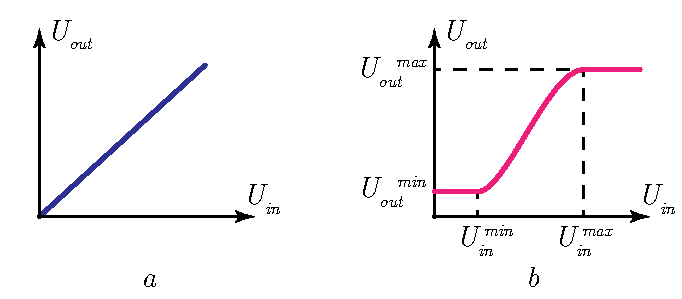
\includegraphics[width=0.8\linewidth]{figs/amp_char.pdf}
    \caption{Амплитудные характеристики идеального и реального усилителя мощности}
    \label{fig:1.1}
\end{figure}

Однако как наблюдается на практике, АХ усилителей редко бывают линейными,
ввиду множества факторов, обуславливающих нелинейность этой характеристики
(см. Рис. \ref{fig:1.1}б). При достаточно больших значениях входной
амплитуды, АХ отклоняется от прямой. Из-за выхода рабочей точки
отдельных элементов усилителя за пределы рабочего диапазона, возникают
нелинейные искажения, вследствие которых коэффициент усиления сигнала
выходит на уровень насыщения.

При этом, АХ реального УМ имеет определенный диапазон входных значений
амплитуд, при которых искажения практически
отсутствуют и усилитель подобен идеальному.
% Эта область называется\textit{динамическим диапазоном усилителя}.
% и выражается как
% \begin{equation}
%     D = \frac{U_{in}^{max}}{U_{in}^{min}}.
% \end{equation}
Одной их характеристик нелинейности является точка сжатия на 1 дБ (P1dB) – точка в
которой реальное усиление становиться на 1 дБ меньше идеальной
характеристики. Измеряется в мощности, в дБм (dBm), равна входному уровню,
при котором выходной уровень становиться на 1 дБ ниже ожидаемого значения
согласно идеальной характеристики.


В связи с ограниченностью линейного диапазона УМ, часто изменяют
входной сигнал таким образом, чтобы итоговая рабочая точка находилась в
нужной области линейности и усиления. Используется смещение рабочей точки
относительно выходной мощности - OBO (\textit{Англ. - Output back-off}), и
смещение рабочей точки относительно входной мощности - IBO (\textit{Англ. -
Input back-off})(см. рис. \ref{fig:obo_ibo}). При этом обычно
представляется возможным пересчет одной величины в другую, так как по сути
они являются взаимозаменяемыми. Разница состоит в том, относительно чего
происходит сдвиг рабочей точки — максимальной выходной, либо максимальной
входной мощности (или P1dB).

\begin{figure}[h!]
    \centering
    \includegraphics[width=0.7\linewidth]{figs/pa_obo_ibo.png}
    \caption{Смещение рабочей точки усилителя относительно входной (IBO) и выходной мощности (OBO).}
    \label{fig:obo_ibo}
\end{figure}

\begin{equation}
    OBO = 10 \cdot \log_{10}\left(\frac{P_{sat}}{P_{out}}\right), \quad
    IBO = 10 \cdot \log_{10}\left(\frac{P_{0}}{P_{in}}\right)
\end{equation}

Большие значения IBO\slash OBO могут обеспечить хорошую линейность АХ,
однако это также приведет к уменьшению средней выходной мощности сигнала.
Таким образом, в реальных применениях определяется наиболее подходящее
значение IBO \slash OBO, обеспечивающее необходимую линейность
характеристики, а также необходимое усиление.


\subsection{Нелинейность и искажение сигналов}
Мощность на выходе УМ увеличивается вместе с ростом входной мощности,
однако, как только уровень выходной мощность достигает определенного
максимума, КУ перестает быть постоянным и усилитель входит в область
насыщения. В этой области больше всего проявляется нелинейность УМ —
выходная мощность перестает увеличиваться с ростом входной мощности. Работа
УМ в нелинейной области влечет за собой нелинейные искажения сигнала,
которые заключаются в изменение его формы и фазы.

В качестве входного рассмотрим сигнал с гармонически меняющейся амплитудной
(мощностью $P_{in}$) (см. рис \ref{fig:pa_distortion_sin}). Если УМ
находится в линейном режиме работы, то на выходе также будет гармонический
сигнал, отличающаяся только усилением амплитуды. Однако если усилитель
находится в нелинейной области, на выходе сигнал будет отличаться от
входного не только значением амплитуды, но и формой. Пики синусоиды будут
сжиматься нелинейной частью АХ, что приведет к искажению сигнала на выходе
(см. рис \ref{fig:pa_distortion_sin}).

\begin{figure}[h!]
    \centering
    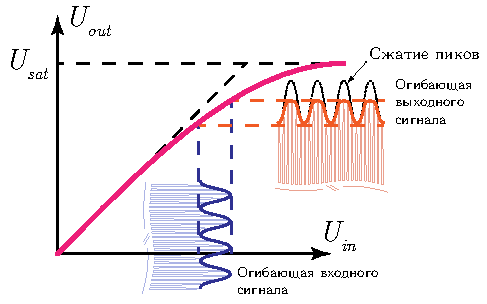
\includegraphics[width=0.6\linewidth]{figs/amp_dist_obo.pdf}
    \caption{Преобразование сигнала с гармонически меняющейся амплитудой при прохождении через УМ}
    \label{fig:pa_distortion_sin}
\end{figure}

% А вот хер знает, тут не уверен

% Сжатие пиков во временной области будет также приводить к искажениям и
% изменениям в частотной области, а именно к росту ширины спектра. Изначально
% подаваемый сигнал имеет очень узкий спектр (дельта-функция на несущей
% частоте) 

% \begin{figure}[h!]
%     \centering
%     \includegraphics[width=0.9\linewidth]{figs/pa_spectral_growth.png}
%     \caption{Влияние сжатия пиков на частотную область сигнала}
%     \label{fig:pa_distortion_freq}
% \end{figure}

Рассмотрим влияние нелинейности характеристики усилителя на основные типы
сигналов, часть которых используется в стандарте 5G NR.

\begin{figure}[h!]
    \centering
    \includegraphics[width=0.98\linewidth]{figs/ofdm_pa_distortions.png}
    \caption{Искажение различных сигналов на приемнике при внесении нелинейного
    искажения на передатчике}
    \label{fig:lls_rapp_distortions_0}
\end{figure}

Для примера рабочая точка (средняя входная мощность) была выбрана так,
чтобы влияние нелинейности амплитудной характеристики усилителя была
достаточно явна продемонстрирована.
\subsubsection{Single Carrier}
\begin{figure}[h!]
    \centering
    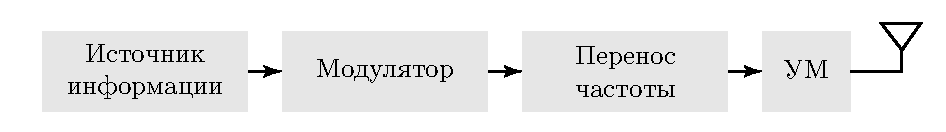
\includegraphics[scale=1]{figs/sc_scheme.pdf}
    \caption{Принципиальная схема генерации SC-сигнала}
    \label{fig:sc_scheme}
\end{figure}
\textit{Single Carrier} - SC сигнал с одной несущей, передаваемые данные
кодируются с помощью модуляции (BPSK, QPSK, N-QAM) в виде амплитуды сигнала
на несущей частоте. Схема генерации SC-сигнала приведена на рис.
\ref{fig:sc_scheme}. Отметим, что SC сигналом часто называют SC-FDMA
сигнал, который в стандарте 5G-NR получил название DFT-s-OFDM.

Поскольку на усилитель подается, по сути, амплитудно модулированный сигнал,
то искажения имеют достаточно предсказуемый характер. На рис.
\ref{fig:lls_rapp_distortions_0}a приведен график созвездия модуляции
64-QAM, который в данном случае используется для сигнала SC. Черные точки
показывают изначальное местоположение созвездия, красные — созвездия на
приемнике с использованием идеального усилителя мощности, синие — созвездия
на приемнике с использованием нелинейного усилителя мощности. 

Наблюдаемая картина напоминает искажение амплитуды на рис.
\ref{fig:pa_distortion_sin}, т.е. искажение обработанного сигнала напрямую
связано с его амплитудой — чем больше амплитуда, тем больше искажение.
Такой тип сигнала имеет детерминированный характер искажения нелинейностью,
и может, в теории, быть достаточно просто компенсирован.


\subsubsection{OFDM / CP-OFDM}
\textit{Orthogonal Frequency-Division Multiplexing} - OFDM сигнал,
использующий большое число близко расположенных ортогональных поднесущих,
каждая из которых модулируется по стандартной схему модуляции (аналогично
SC). В стандарте 5G NR часто используется \textit{CP}-OFDM - \textit{Cyclic
Prefix} OFDM - сигнал OFDM с добавлением цикличного префикса. CP необходим
для борьбы с межсимвольной интерференцией (ISI), и заключается в создании
межсимвольного защитного интервала, состоящего из копии части
OFDM-символа. Принципиальная схема генерации OFDM сигнала приведена на рис.
\ref{fig:ofdm_scheme}. OFDM сигнал принципиально отличается от SC сигнала,
поток данных делится на несколько параллельных подпотоков с более низкой
скоростью передачи (увеличение длительности символа), а каждый поток
модулируется на своей ортогональной поднесущей. OFDM также достаточно прост
в обработке, чаще всего применяется прямое и обратное преобразование Фурье,
с помощью которого происходит перенос сигнала между частотной и временной
областью.
\begin{figure}[h!]
    \centering
    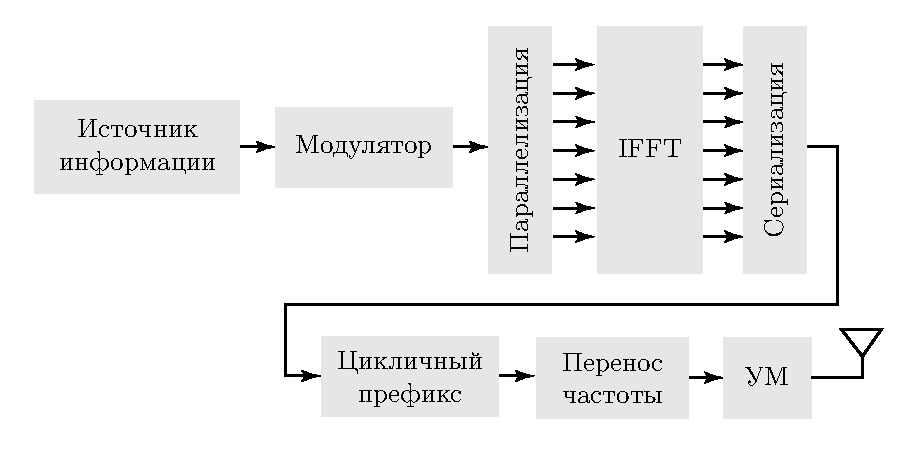
\includegraphics[scale=1]{figs/ofdm_scheme.pdf}
    \caption{Принципиальная схема генерации CP-OFDM-сигнала.
    \textbf{M}-IFFT означает что операция IFFT производится по M точкам.}
    \label{fig:ofdm_scheme}
\end{figure}

Что касается искажения при прохождении через нелинейный УМ, ввиду наличия
операции IFFT (на передатчике) перед усилителем, результирующие искажения
на приемнике после преобразования OFDM-сигнала в созвездие с помощью FFT
имеют достаточно сложный и непредсказуемый характер, как и это предложение.
Пример искажений OFDM-сигнала изображен на рис.
\ref{fig:lls_rapp_distortions_0}b. Из графика видно, что размер облака
точек вокруг точек созвездий увеличивается при присутствии нелинейного
усилителя в цепи передатчика (синие точки), однако отсутствует
централизованный сдвиг облаков относительно изначальных положений. 

Таким образом, искажения CP-OFDM сигнала носят недетерминированный
характер, в какой-то степени случайный. Такие искажения может быть
проблематично компенсировать.

\subsubsection{DFT-s-OFDM}
\textit{(Discrete) Fourier Transform Spread OFDM} - DFT-s-OFDM сигнал
является модификацией сигнала OFDM, нацеленной на компенсацию его основного
недостатка, а именно высокого отношения пикового уровня мощности к среднему
(\textit{Англ. - Peak to Average Power Ratio - PAPR}). Подробнее проблема
высокого PAPR рассмотрена в секции \ref{sec:papr}. Принципиальная схема
генерации DFT-s-OFDM сигнала приведена на рис. \ref{fig:dfts_scheme}.
\begin{figure}[h!]
    \centering
    % 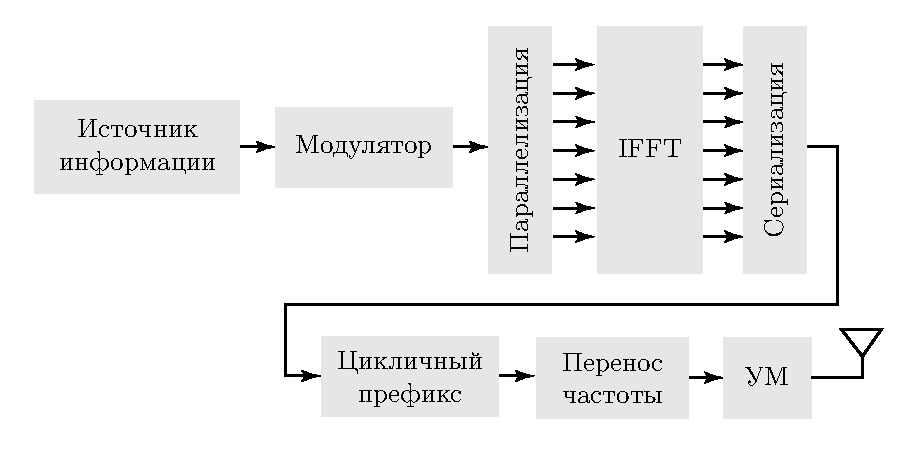
\includegraphics[scale=1]{figs/ofdm_scheme.pdf}
    % \includegraphics[scale=0.8]{example-image-a}
    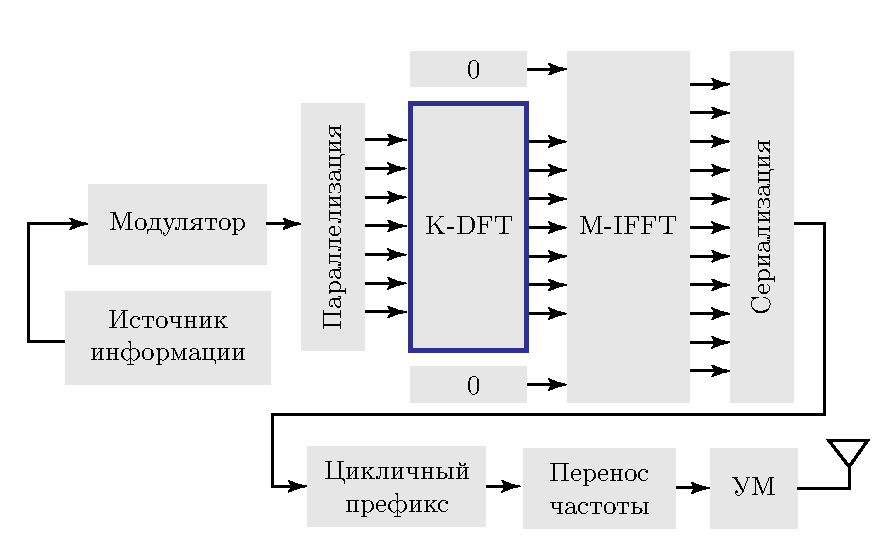
\includegraphics[scale=1]{figs/dfts_scheme.pdf}
    \caption{Принципиальная схема генерации DFT-s-OFDM-сигнала.
    \textbf{K}-DFT означает что операция DFT производится по K точкам.}
    \label{fig:dfts_scheme}
\end{figure}
Генерация DFT-s-OFDM сигнала отличается от классического OFDM включением
предварительного кодирования параллелизованного потока данных при помощи
прямого дискретного преобразования Фурье (DFT, FFT), примененного к
ограниченному количеству поднесущих OFDM сигнала ($K<M$). В стандарте 3GPP
данная операция называется \textit{Transform Precoding}. По своей сути
эта процедура повторяет принцип, применяемый в SC-FDMA. За счет
сочетания Transform Precoding и IFFT, присутствующего в процедуре создания
OFDM сигнала, полученный сигнал имеет меньшие значения PAPR, тем самым
более эффективно используя ограниченный диапазон работы усилителя.

Поскольку DFT-s-OFDM сигнал является неким средним между CP-OFDM и SC,
искажения, вносимые нелинейностью УМ имеют также смешанный характер. Пример
таких искажений приведен на рис. \ref{fig:lls_rapp_distortions_0}c.
Присутствует как общее смещение облаков созвездия ввиду амплитудных
искажений, так и увеличение разброса по сравнению со случаем
использования идеального (линейного) усилителя.

\subsection{Проблема пик-фактора PAPR сигнала OFDM}
\label{sec:papr}
Одним из недостатков сигнала OFDM является высокое отношение пиковой
мощности к средней - PAPR (пик-фактор). Визуализация этого отношения приведена на рис.
\ref{fig:papr}. В случае OFDM сигнала, высокое значение PAPR получается в
результате комбинации большого количества поднесущих, которые могут
когерентно сложиться, что и даст высокое значение пиковой мощности.
 
\begin{figure}[h!]
    \centering
    % 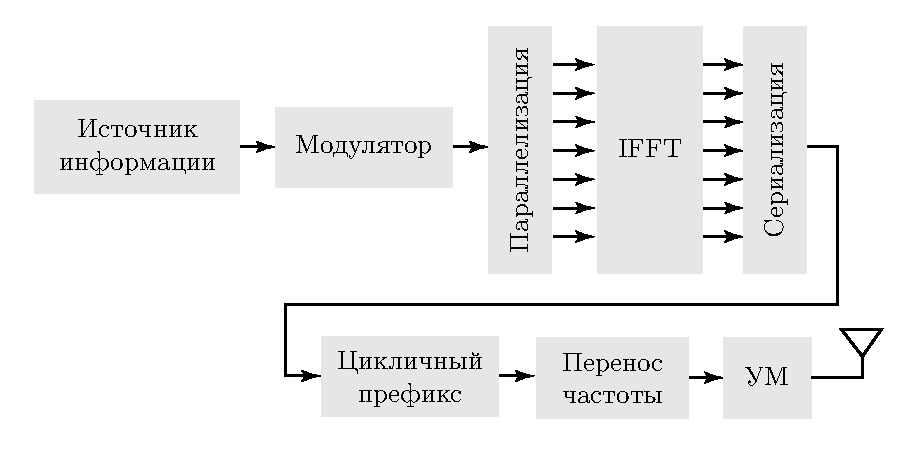
\includegraphics[scale=1]{figs/ofdm_scheme.pdf}
    % \includegraphics[width=0.49\linewidth]{figs/papr_scheme.png}
    % \includegraphics[width=0.49\linewidth]{figs/papr_ofdm.png}
    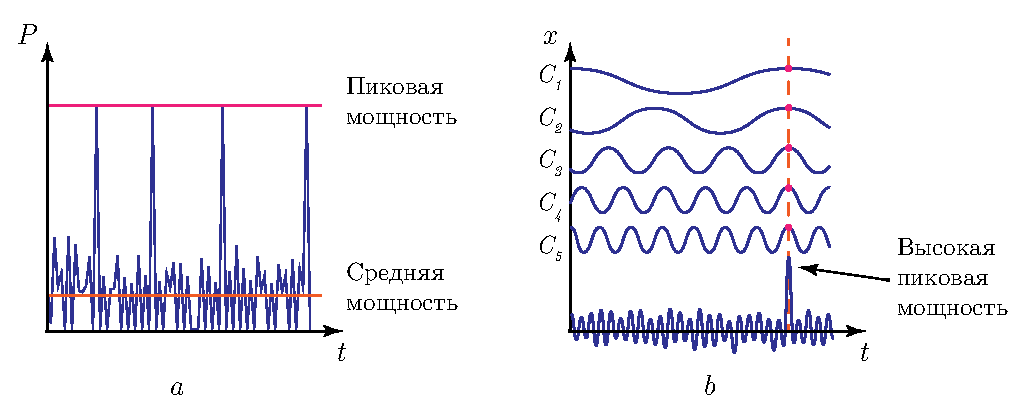
\includegraphics[scale=1]{figs/papr_explanation.pdf}
    \caption{Демонстрация отношения пиковой мощности сигнала к средней
    мощности (слева) и принцип появления высокого PAPR у OFDM
    сигнала (справа). При комбинации большого количества гармоник возможно
    их сложение в фазе, что приведет к скачку мощности.}
    \label{fig:papr}
\end{figure}
Высокое значение PAPR негативно влияет на работу системы в целом, поскольку
напрямую влияет на выбор рабочей точки усилителя. Перед подачей на УМ,
сигнал должен быть настроен таким образом, чтобы его средняя мощность,
определяющая рабочую точку, соответствовала желаемому режиму работы
усилителя. Если отношение PAPR высокое, то при выбранной на основе средней
мощности рабочей точки, части сигнала с пиковой мощностью будут попадать на
сильно нелинейную часть характеристики усилителя, что приведет к
искажению. Для избежания негативных эффектов, часто сдвигают рабочую точку
таким образом, чтобы сигнал не искажался, однако вместе с этим также
понижается общая выходная мощность.

В стандарте LTE при передаче данных от пользователя к базовой станции
(\textit{Uplink}) используется сигнал SC-FDMA \cite{3gpp.36.211}, поскольку
высокое значение пик-фактора на мобильных устройствах не приемлемо. В
стандарте 5G NR, в качестве альтернативы OFDM в uplink используется сигнал
DFT-s-OFDM \cite{3gpp.38.300}. Эти сигналы отличаются пониженным значением
пик фактора \cite{Vaigandla2021}, что позволяет более эффективно
использовать УМ.


\subsection{Математическое описание характеристик реальных УМ}

Для моделирования использования УМ в системах мобильной связи часто прибегают к
математическим моделям, описывающим поведение сигнала (усиление, искажение) при 
прохождении через УМ. Исторически модели разделяются на две основных
группы — \textbf{физические} и \textbf{эмпирические} модели \cite{cambridge2008}.

Физические модели требуют знания внутренних электронных компонентов УМ, их
связи, а так же теории, описывающей их взаимодействие. Такие модели подходят
для симуляций на уровне схемы благодаря высокой точности, однако требуют
много вычислительных мощностей и времени, а также детальное описание
структуры и компонентов УМ.

Эмпирические модели используются, когда не известна внутренняя структура УМ,
или когда рассматривается системный уровень моделирования. Эти модели
основаны на результатах измерений и исследований конкретных УМ, на основе
которых были выведены зависимости снятых характеристик УМ (АХ, ФХ) от его
параметров.

Поскольку в данной работе исследуется возможность компенсации нелинейного
искажения на приемнике, то использоваться будет эмпирическая
(поведенческая) модель УМ. Среди таких моделей можно назвать
\textit{Volterra, Saleh, Ghorbani}, а также модели, представляющие собой комбинации
полиномиальных моделей. Все они являются достаточно простыми моделями,
которые отражают нелинейную природу УМ. Простота позволяет оперировать
меньшим количеством параметров усилителя, упрощая обработку в целом. Однако
такие модели не могут быть использованы для описания сложных усилителей,
таки как усилитель \textit{Doherty} \cite{Doherty1936}\cite{3gpp.38.803}.

С другой стороны, в рамках рассматриваемой задачи, а именно компенсации
искажений, внесенных на передатчике из-за нелинейности УМ, использование
более простой модели может быть оправдано. Целью данной работы является
создание метода компенсации нелинейных искажений на приемнике, с основным
мотивом минимизировать обработку на передатчике, а также стоимость
конечного устройства. Рассматриваются именно простые, мало размерные,
дешевые в производстве передатчики, в которых усилитель часто имеет далеко
не лучшие параметры и не отличается высокой эффективностью.

\subsubsection{Модель Раппа}
\begin{figure}[h!]
    \centering
    \includegraphics[width=0.7\linewidth]{figs/rapp_p.png}
    \caption{Влияние параметра гладкости $p$ на вид амплитудной
    характеристики
    % (Добавить вторую и третью картинку где будут менять G, V)
    }
    \label{fig:rapp_p_parameters}
\end{figure}
Для описания искажения амплитуды и фазы при использовании твердотельных УМ
широко используется модель Раппа (\textit{Англ. - Rapp}) \cite{Rapp1991} \cite{Maltsev2010}.
Также существует модифицированная модель Раппа, приведенная в выражении
\ref{eq:Rapp}. Данная модель УМ включена в список моделей в спецификации
3GPP \cite{3gpp.38.803}.

\begin{equation}
    F_{AM/AM}(x) = \frac{G x}{\left( 1 + \abs{\frac{Gx}{V_{sat}}}^{2p}\right)^{1/2p}},
    \quad 
    F_{AM/PM}(x) = \frac{Ax^q}{\left(1+\left(\frac{x}{B}\right)^q\right)},
    \label{eq:Rapp}
\end{equation}
где $F_{AM/AM}, F_{AM/PM}$ - амплитудные и фазовые характеристики
соответственно, $G$ - КУ слабого сигнала, $V_{sat}$ - амплитуда насыщения,
$p$ - показатель гладкости характеристики. Параметры $A,B,q$ - параметры
кривой искажения фазы. В дальнейшем в работе будет использоваться эта
модель для описания влияния УМ на сигнал.

Пример АХ и ФХ для модели Раппа приведены на  рис. \ref{fig:rapp_p_parameters}.
В зависимости от значений параметров $G, V_{sat}, p$ поведение амплитудной
характеристики может сильно варьироваться. Так, при больших значениях $p$
($p\gg 1$), АХ похожа на характеристику идеального УМ, которая ограничена
по максимальной выходной амплитуде (см. рис. \ref{fig:rapp_p_parameters}).
Параметр $V_{sat}$ отвечает за выходную амплитуду насыщения, а $G$ - КУ
слабого сигнала.


\subsubsection{Параметры модели Раппа для диапазона 30-70 ГГц}
Для вывода параметров базовой модели УМ в диапазоне частот 30-70 ГГц,
компанией Nokia были использованы и исследованы характеристики стандартных
усилителей в соответствующей полосе \cite{nokia163314} \cite{Maltsev2010}.
Полученная модель УМ использована в этой работе для моделирования влияния
нелинейности УМ для сигналов с несущей частотой в диапазоне 30-70 ГГц.
Амплитудные и частотные характеристики УМ в соответствии с моделью
\cite{nokia163314} для 30-70 ГГц приведены на рис. \ref{fig:rapp_nokia}.
Численные значения параметров модели Раппа приведены в \ref{eq:rapp_p3070}.

\begin{equation}
    G = 16, \quad V_{sat} = 1.9, \quad p = 1.1
    \label{eq:rapp_p3070}
\end{equation}

\begin{figure}[h!]
    \centering
    \includegraphics[width=0.7\linewidth]{figs/rapp_nokia.png}
    \caption{АХ и ФХ усилителя в соответствии с моделью Раппа и
    параметрами для диапазона 30-70 ГГц}
    \label{fig:rapp_nokia}
\end{figure}

\subsection{Характеристики УМ в миллиметровом диапазоне}
Помимо исследования диапазона частот 30-70 ГГц, в рамках данной работы
рассматривалось влияние нелинейного усилителя на качество приема для
диапазона миллиметровых длин волн, а именно 100-200 ГГц. Поскольку на
момент проведения исследования модель УМ для данного диапазона
отсутствовала, были изучены многочисленные отчеты и исследования с
указанием амплитудных характеристик используемых усилителей. Основываясь на
работах \cite{zhang2021}\cite{amadorey2018}\cite{aliyun2020} был сделан
вывод о значительном отличии характеристик УМ в более высоком диапазоне
частот. В целом, рассматриваемые усилители имею значительно меньшее
значение амплитуды насыщения $V_{sat}$ (или мощности насыщения), а также
меньшее значение коэффициента усиления $G$.

Характеристики твердотельных УМ из работ
\cite{zhang2021}\cite{amadorey2018}\cite{aliyun2020} приведены на рис.
\ref{fig:pa_research_mean}. Также на рис. \ref{fig:pa_research_mean}
приведена модель для 30-70 ГГц.
\begin{figure}[h]
    \centering
    \includegraphics[width=0.95\linewidth]{figs/pacomparison.png}
    \caption{АХ усилителей на основе данных из
    \cite{zhang2021}\cite{amadorey2018}\cite{aliyun2020}, а также
    модель 30-70 ГГц \cite{nokia163314} и полученная усредненная модель
    для диапазона 100-200 ГГц}
    \label{fig:pa_research_mean}
\end{figure}

Извлеченные кривые амплитудных характеристик были аппроксимированы при
помощи модели Раппа \ref{eq:Rapp} (см. рис. \ref{fig:pa_research_mean} -
пунктирные линии), что позволило собрать параметры УМ для дальнейшей
обработки. Полученные значения параметров модели, а также частота и
технология для рассматриваемых усилителей приведены в Таблице
\ref{tab:pa_params}. 

\begin{table}[h]
    \centering
    \begin{tabular}{llcccc}
        \hline
    Источник              & Технология   & Частота, ГГц & $G$  & $V_{sat}$ & $p$ \\ \hline
    \cite{zhang2021}      & 28-нм CMOS   &  135         & 12.26 & 0.9      & 1.93  \\
    \cite{amadorey2018} Рис. 6.2b  & 35-нм mHEMT      &  180  & 10.84 & 0.87 & 0.52 \\
    \cite{amadorey2018} Рис. 6.4b  & 50-нм mHEMT      &  198  & 41.19 & 1.99 & 0.26  \\
    \cite{amadorey2018} Рис. 6.15a & 35-нм GaAs mHEMT &  210  & 7.89  & 0.44 & 0.9  \\
    \cite{aliyun2020} CT       &  130-нм SiGe BiCMOS CT        & 185 & 2.05  & 1.09 & 2.03  \\
    \cite{aliyun2020} CE       & 130-нм SiGe BiCMOS CE         & 185 & 4.08  & 1.41 & 1.91  \\
    \cite{aliyun2020} Рис. 19a & 130-нм SiGe BiCMOS 3-stage CT & 160 & 9.88  & 1.81 & 2.75  \\
    \cite{aliyun2020} Рис. 19b & 130-нм SiGe BiCMOS 3-stage CT & 170 & 14.8  & 1.81 & 1.56  \\
    \cite{aliyun2020} Рис. 19c & 130-нм SiGe BiCMOS 3-stage CT & 185 & 19.29 & 1.86 & 0.87  \\\hline
    \end{tabular}
    \caption{Параметры модели Раппа для УМ в диапазоне частот 100-200 ГГц
    на основе экспериментальных данных и исследований}
    \label{tab:pa_params}
\end{table}

\subsubsection{Параметры новой модели для диапазона частот 100-200 ГГц}
Для исследования применимости нового метода компенсации в диапазоне 100-200
ГГц необходима соответствующая модель УМ, для начальной имплементации ее в
систему с целью внесения соответствующих искажений в сигнал, и последующей
компенсацией внесенных искажений на приемнике. 

Имеющаяся модель \cite{nokia163314} подходит только для диапазона  30-70
ГГц, в нашем случае интерес представляет работа при более высоких частотах.
Модель для 100-200 ГГц была создана путем усреднения параметров $G,
V_{sat}, p$ рассмотренных УМ в соответствующем диапазоне частот (см. Таблицу
\ref{tab:pa_params}). Полученные усредненный параметры для модели Раппа
приведены в \ref{eq:rapp_p100200}.
\begin{equation}
    G = 13.59, \quad V_{sat} = 1.35, \quad p = 1.41
    \label{eq:rapp_p100200}
\end{equation}
Усредненная характеристика была получена только для амплитудного искажения $F_{AM/AM}$,
модель фазовых искажений была выбрана аналогичной модели для 30-70 ГГц.


\section{Метод компенсации нелинейных искажений на приемнике}
Компенсация нелинейных искажений сигнала является важным этапом для
сохранения производительности системы. С расширением стандарта связи 5G NR
в миллиметровый диапазон, компенсация становится особенно актуальной,
поскольку характеристики усилителей в этом диапазоне значительно хуже, чем
для более низких частот.

\subsection{Обзор существующих решений}
На текущий момент были исследованы несколько основных подходов для
компенсации нелинейных искажений, они разделяются на два основных
направления. Первый заключается в предварительном искажении сигнала перед
подачей на УМ на передатчике. Сигналу придаются свойства, которые
минимизируют влияние нелинейного искажения от УМ, эффективно "выпрямляя"
его АХ. Существует множество вариантов обработки для данного подхода,
однако многие из них имеют слабый эффект на общей производительности
системы, а подход с применением предварительного искажения сигнала имеет
низкую эффективность при низких значениях IBO, при которой достигается
максимальная эффективность усилителя \cite{sharath2015}
\cite{shabany2008} \cite{eda2001}. Также, использование PD на передатчике
нежелательно на мало-габаритных устройствах, поскольку в таком случае
увеличивается сложность устройства, объем сигнальной обработки и энергопотребление.


Второй основной подход заключается в компенсации нелинейных искажений на
приемнике. Например, в работе \cite{maltsev2021} используется
статистическая обработка принятого сигнала для определения степени
искажения, на основе которой в дальнейшем производится компенсация. Многие
работы \cite[]{sharath2015, shabany2008,bhat2016,qi2010,gregorio2007,
bouhadda2015,drotar2010} рассматривают теоретический подход для компенсации
на приемнике в очень обобщенном случае. Несколько методов компенсации были
предложены для OFDM сигнала \cite[]{gregorio2007,bouhadda2015, drotar2010},
где влияние нелинейности представляется комплексным множителем, а также
Гауссовой шумовой компонентой. Основной задачей в таком случае является
определение параметров УМ (они могут быть как известны изначально, так и
определены с помощью пилотных сигналов) для компенсации нелинейного
искажения. Несколько методов были исследованы для сигнала SC с одной несущей
(\textit{Англ. - SC - Single Carrier}) \cite[]{sharath2015,
shabany2008,bhat2016, qi2010}, в частности использовалась обратная
характеристика УМ и последовательные методы Монте-Карло. В нескольких
случаях \cite[]{bhat2016, qi2010,gregorio2007}, значения параметров УМ
считаются известными на приемнике, что позволяет произвести компенсацию
искажения. В случаях, когда параметры УМ оцениваются, производительность
такая же либо хуже.

В данной работе описывается метод компенсации нелинейных искажений УМ на
приемнике с использованием обратной амплитудной характеристики. Информация
о параметрах и рабочей точке усилителя предполагается известной. Работа и
эффективность метода будет исследоваться на существующем симуляторе
канального уровня, необходимые изменения будут вноситься в код симулятора
как для внесения искажений, так и для их компенсации.



\subsection{Краткое описание архитектуры LLS}

Для исследования влияния нелинейности УМ в диапазонах частот 30-70 ГГц и
100-200 ГГц, а также проверки работоспособности разработанного метода
компенсации нелинейных искажений на приемнике, в работе использовался
полноценный симулятор канального уровня LLS (\textit{Англ. - Link Level
Simulator}), соответствующий требованиям стандарта 5G NR 3GPP. В этой части
работы будут кратко описаны принципы работы, архитектура и основные
составляющие LLS. 

На рис. \ref{fig:lls_scheme} приведена принципиальная схемы работы LLS.
\begin{figure}[h!]
    \centering
    \includegraphics[width=0.99\linewidth]{figs/lls_scheme.png}
    \caption{}
    \label{fig:lls_scheme}
\end{figure}

TBD

% Схема компенсации состоит из базовой обработки на передатчике (1),
% которая может включать MIMO прекодинг и transform прекодинг (в случае
% DFT-s-OFDM сигнала),  а также стандартного для OFDM блока обратного
% преобразования Фурье. Сгенерированный OFDM сигнал подается на одну или
% более передающих цепочек, которые могут включать добавление цикличного
% префикса, перенос сигнала на несущую частоту, и, наконец, сигнал подается
% на усилитель мощности (2), работающий на несущей частоте. Отметим, что
% для корректной работы предлагаемой схемы, сигналы на разных антеннах
% должны иметь одинаковую амплитуду (но могут иметь разную фазу). Это
% ограничивает применение данного метода до передачи 1 ранга, даже если
% используется несколько передающих антенн. После прохождения через канал,
% сигнал попадает на приемную цепь состоящую из одной или нескольких
% приемных антенн для дальнейшей обработки (4), которая может состоять из
% преобразования Фурье further maximum ration combining (MRC) and frequency
% domain equalization???. Такая обработка эффективно нивелирует влияние
% частотно-селективного канала, что позволяет использовать обработанный
% сигнал на блоке компенсации нелинейного искажения (5). Этот блок может
% состоять из операции обратного Фурье преобразования (6) для возвращения
% сигнала во временную область, блока обратной нелинейной функции УМ (7),
% который выполняет компенсацию нелинейного искажения, а также блока
% прямого преобразования Фурье для возвращения сигнала в частотную область.






\subsection{Влияние нелинейных искажений в LLS}

\begin{figure}[h!]
    \centering
    \includegraphics[width=0.95\linewidth]{figs/ofdm_pa_distortions.png}
    \caption{Искажение различных сигналов на приемнике при внесении нелинейного
    искажения на передатчике}
    \label{fig:lls_rapp_distortions}
\end{figure}

\subsection{Подход и описание нового метода компенсации нелинейных искажений}
В основе разработанного метода компенсации нелинейных искажений на
приемнике лежит использование обратной АХ усилителя. Параметры $G, V_{sat},
p$, необходимые для восстановления обратной характеристики считаются
известными. Помимо этих параметров, важно также знать рабочую точку УМ,
поскольку это напрямую влияет на степень искажения принятого сигнала.
Рабочая точка также считается известной.

Принципиальный подход компенсации искажений может быть описан следующим
образом:
\begin{enumerate}
    \item Принятый сигнал проходит через предварительную обработку в LLS
    (частотное выравнивание, MIMO-декодирование, перенос в частотную
    область)
    \item Полученный обработанный сигнал в частотной области переносится во
    временную область в соответствии с используемым типом сигнала.
    \subitem Transform precoding (в случае DFT-s-OFDM сигнала)
    \subitem IFFT-обработка для получения OFDM сигнала во временной области
    \item Полученный сигнал во временной области подается на блок
    компенсации (использующий обратную АХ усилителя на основе известных
    параметров и рабочей точки)
    \item Сигнал с компенсированными искажениями переводится в частотную
    область
    \item Компенсированный сигнал подается на блок демодуляции
\end{enumerate}

Блок-схема разработанного метода компенсации приведена на рис.
\ref{fig:compensation_scheme}. 

\begin{figure}[h!]
    \centering
    \includegraphics[width=0.95\linewidth]{figs/compensation_scheme.png}
    \caption{}
    \label{fig:compensation_scheme}
\end{figure}

\begin{equation}
    F^{-1}_{AM/AM}(y) = 
    \begin{cases}
        \displaystyle
       \frac{ y}{\left( 1 - \abs{\frac{y}{V_{sat}}}^{2p}\right)^{1/2p}}
       \quad y <\alpha V_{sat}\\
       \frac{ \alpha V_{sat}}{\left( 1 - \abs{\alpha}^{2p}\right)^{1/2p}}
       \quad y \geq \alpha V_{sat}
    \end{cases},
    \label{eq:invRapp}
\end{equation}

TBD



\subsubsection{Компенсация с использованием обратной характеристики усилителя}
Тут написать про обратную характеристику, приколы возникающие при ее
неограничении и как она используется для компенсации.

\subsubsection{Адаптация алгоритма компенсации в зависимости от типа используемого сигнала}
Возможность обработки нескольких типов сигнала в зависимости от типа
сигнала.
\section{Результаты}
To prove the feasibility of the proposed approach, link-layer simulations
(LLS) were performed, comparing the proposed scheme with the cases of ideal
PA and no-compensation case for a given PA model. The model based
parameters of the typical real power amplifiers in the 30-70 GHz band [15]
was used along with newly developed model for the 100-200 GHz. Basic LLS
simulation assumptions are summarized in Table 1.

\begin{figure}[h!]
    \centering
    \includegraphics[width=0.5\linewidth]{figs/parameters table.png}
\end{figure}

\subsection{Результаты симуляций для модели 30-70 ГГц}

\begin{figure}[h!]
    \centering
    \includegraphics[width=0.49\linewidth]{figs/res/ofdm/OFDM_Nokia_SCS120_MCS22_27.png}
    \includegraphics[width=0.49\linewidth]{figs/res/dftsofdm/DFT-s-OFDM_Nokia_SCS120_MCS22_27.png}
    \caption{BLER for SCS 120 kHz, 64-QAM/256 QAM for OFDM (left) and DFT-s-OFDM(right)}
    \label{fig:res3070_scs120}
\end{figure}

\begin{figure}[h!]
    \centering
    \includegraphics[width=0.49\linewidth]{figs/res/ofdm/OFDM_Nokia_SCS480_MCS22_27.png}
    \includegraphics[width=0.49\linewidth]{figs/res/dftsofdm/DFT-s-OFDM_Nokia_SCS480_MCS22_27.png}
    \caption{SCS480}
    \label{fig:res3070_scs480}
\end{figure}

\begin{figure}[h!]
    \centering
    \includegraphics[width=0.49\linewidth]{figs/res/ofdm/OFDM_Nokia_SCS960_MCS22_27.png}
    \includegraphics[width=0.49\linewidth]{figs/res/dftsofdm/DFT-s-OFDM_Nokia_SCS960_MCS22_27.png}
    \caption{SCS960}
    \label{fig:res3070_scs960}
\end{figure}

\subsection{Результаты симуляций для модели 100-200 ГГц}

\begin{figure}[h!]
    \centering
    \includegraphics[width=0.49\linewidth]{figs/res/ofdm/OFDM_SubTHz_SCS120_MCS22_27.png}
    \includegraphics[width=0.49\linewidth]{figs/res/dftsofdm/DFT-s-OFDM_SubTHz_SCS120_MCS22_27.png}
    \caption{SCS120}
    \label{fig:res100200_scs120}
\end{figure}

\begin{figure}[h!]
    \centering
    \includegraphics[width=0.49\linewidth]{figs/res/ofdm/OFDM_SubTHz_SCS480_MCS22_27.png}
    \includegraphics[width=0.49\linewidth]{figs/res/dftsofdm/DFT-s-OFDM_SubTHz_SCS480_MCS22_27.png}
    \caption{SCS480}
    \label{fig:res100200_scs480}
\end{figure}

\begin{figure}[h!]
    \centering
    \includegraphics[width=0.49\linewidth]{figs/res/ofdm/OFDM_SubTHz_SCS960_MCS22_27.png}
    \includegraphics[width=0.49\linewidth]{figs/res/dftsofdm/DFT-s-OFDM_SubTHz_SCS960_MCS22_27.png}
    \caption{SCS960}
    \label{fig:res100200_scs960}
\end{figure}


% \subsection{Последовательность применения компенсаций} Предложенный метод
% предполагается использовать до компенсации фазового шума (PN), однако
% другие последовательности были рассмотрены и рассчитаны. Применение
% компенсации нелинейности УМ после компенсации PN показало определенное
% ухудшение производительности, поэтому компенсация нелинейности УМ везде
% производилась до компенсации фазовых шумов в большинстве расчетов.
% Примеры результатов, в которых сравнивается разный порядок компенсации
% фазовых шумов и нелинейности усилителя приведены на Figure 10.

% \subsection{Наблюдения}

% • Для модели УМ в диапазоне 30-70 ГГц (подходящего для диапазона АК2 и
% выше) улучшение наблюдается только для модуляций высокого порядка o Для
% SCS 120 кГц, отрицательные эффекты фазового шума значительны, и при таких
% искажениях результаты компенсации нелинейности УМ незначительны o Для SCS
% 480 и 960 кГц, в которых возможна более эффективная компенсация фазового
% шума, в определенный момент влияние нелинейности УМ становится основным
% ограничивающим фактором. В этом случае компенсация нелинейности УМ может
% улучшить результат на несколько дБ или совсем избавиться от искажений,
% внесенных УМ. • Для модели 100-200 ГГц, влияние нелинейности УМ
% увеличивается, и в большинстве случаев превосходит влияние фазовых шумов
% o Предложенный метод компенсации демонстрирует улучшение результата для
% MCS 22 и выше • Не смотря на возможность различных имплементаций,
% диктуемая логикой последовательность компенсации искажений в порядке,
% обратному их появлению в системе оказывается оптимальным. Таким образом,
% искажения должны быть компенсированы в порядке канал, усилитель мощности,
% фазовые шумы.  
\section{Заключение}

% Описан и продемонстрирован метод для компенсации нелинейных искажений
% усилителя мощности на стороне приемника. В основе метода лежит
% использование обратной амплитудной характеристики усилителя, метод может
% быть применен для нескольких различных типов сигнала и подстроен для
% рассматриваемой задачи. Компенсация была реализована и протестирована на
% симуляторе канального уровня, соответствующего требованиям стандарта 5G
% NR для оценки влияния на производительность системы. Метод применялся для
% существующей модели УМ в диапазоне частот 30-70 ГГц, а также для новой
% модели 100-200 ГГц, основанной на последних исследованиях. В обоих
% случаях, предлагаемый метод продемонстрировал возможность значительно
% улучшить производительность системы в различных условиях (вид сигнала,
% модуляция и др.). Поскольку метод опирается на компенсацию на стороне
% приемника, этот подход может быть эффективен в системе с большим
% количеством простых, дешевых передатчиков с низким энергопотреблением.
% Это позволит устройству передачи снизить общее энергопотребление,
% поскольку в таком случае отсутствует необходимость в предварительной
% обработке сигнала для компенсации нелинейных эффектов усилителя.
% \include{sections/5-appendix}


%! TeX root = ../main.tex
\SafetyRules
При выполнении компьютерного моделирования на персональной
ЭВМ соблюдалась техника безопасности в
соответствии с СанПин 2.2.2/2.4.1340-03 \cite{SanPin}.  В помещениях для работы на
компьютерах необходимым условием является наличие естественного и искусственного
освещения.  Естественное освещение реализуется через окна, ориентированные
преимущественно на север и северо-восток. Не допускается размещение мест
пользователей ПЭВМ в цокольных и подвальных помещениях.  Искусственное освещение
должно осуществляться системой общего равномерного освещения. Яркость
светильников в зоне углов излучения от 50 до 90 градусов с вертикалью в
продольной и поперечной плоскостях должна составлять не более 200 кд/м$^2$,
защитный угол светильников должен быть не менее 40 градусов. В случае работы
преимущественно с документами, допускается применение комбинированного
освещения: кроме общего устанавливаются светильники местного освещения, которые
не должны создавать бликов на поверхности экрана и увеличивать его освещенность
более 300 лк.  Площадь одного рабочего места для взрослых пользователей должна
составлять не менее 6 м$^2$, а объем – не менее 20 м$^3$.  Для внутренней отделки
помещений должны использоваться диффузно-отражающие материалы с коэффициентом
отражения от потолка – $0.7–0.8$; для стен – $0.5–0.6$; для пола – $0.3–0.5$.
Поверхность пола в помещениях должна быть ровной, без выбоин, нескользкой,
удобной для очистки и влажной уборки, обладать антистатическими свойствами.
Микроклимат в помещениях, где установлены компьютеры, должен соответствовать
санитарным нормам: температура воздуха в теплый период года должна быть не более
23–25 градусов Цельсия, в холодный – 22–24 градуса Цельсия; относительная
влажность воздуха должна составлять 40–60; скорость движения воздуха – 0.1 м/с.

Для повышения влажности воздуха в помещениях следует применять увлажнители
воздуха, заправляемые ежедневно дистиллированной или прокипяченной питьевой
водой. Помещения перед началом и после окончания работы за компьютером следует
проветривать.  Экран видеомонитора должен находиться от глаз пользователя на
оптимальном расстоянии 600-700 мм, но не ближе 500 мм с учетом размеров
алфавитно-цифровых знаков и символов. При непрерывной работе с компьютером
каждые 1-2 часа делать перерыв на 10-15 минут для отдыха и выполнения комплекса
физкультурно-оздоровительных упражнений.



% \nocite{*}
\newpage
{\footnotesize
\printbibliography
}


\end{document}
